\documentclass[border=10pt]{standalone}

\usepackage{tikz}
\usepackage{tikzsymbols}
\usetikzlibrary{calc,patterns,shapes.geometric}

\def\centerarc[#1](#2)(#3:#4:#5){\draw[#1] ($(#2)+({#5*cos(#3)},{#5*sin(#3)})$) arc (#3:#4:#5);}

\begin{document}
	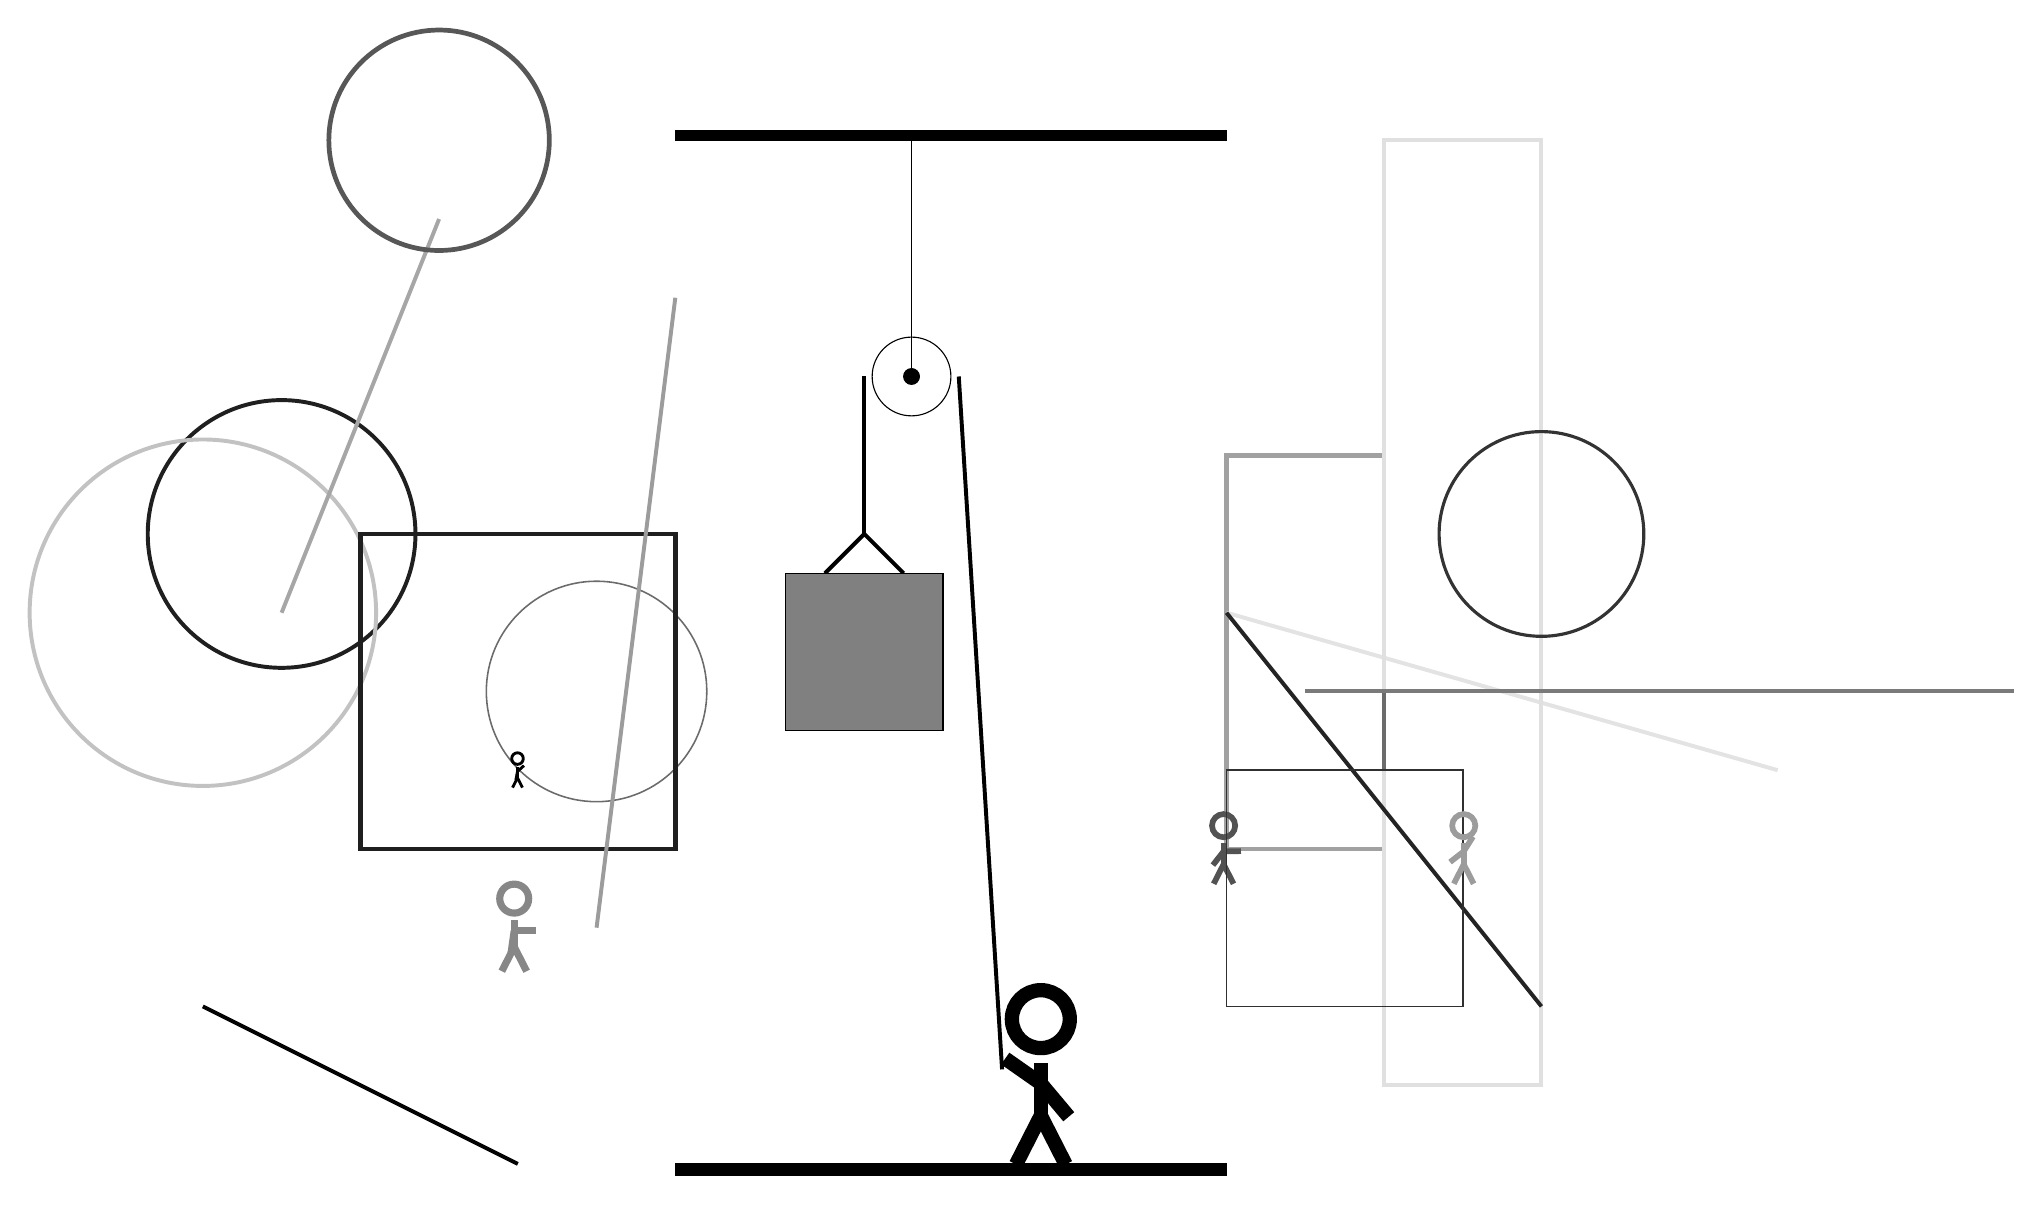
\begin{tikzpicture}
		%%%%% START %%%%%
		
		\draw[fill=black] (-2, 10) rectangle (5, 10.125);
		
		\draw (1, 7) circle (0.5);
		\draw[fill=black] (1, 7) circle (0.1);
		\draw (1, 10) -- (1, 7);
		
		\draw[line width=0.5mm] (-0.1, 4.5) -- (0.4, 5.0) -- (0.9, 4.5);
		\draw[fill=black!50] (-0.6, 4.5) rectangle (1.4, 2.5);
		
		\draw[line width=0.5mm] (0.4, 7) -- (0.4, 5.0);
		\centerarc[line width=0.5mm](1, 7)(0:180:0.6);
		\draw[line width=0.5mm](1.6, 7) -- (2.15, -1.8);
		
		\node at (2.6, -1.9) {\Strichmaxerl[10][-35][-50]};
		
		\draw [line width=0.5mm, color=black!88](-7, 5) circle (1.7);
		
		\draw[line width=0.6mm, color=black!37] (5, 1) rectangle (7, 6);
		\draw [line width=0.5mm, color=black!24](-8, 4) circle (2.2);
		\draw [line width=0.2mm, color=black!58](-3, 3) circle (1.4);
		\draw[line width=0.5mm, color=black!11](5, 4) -- (12, 2);
		\draw[line width=0.5mm, color=black!99](-4, -3) -- (-8, -1);
		
		\node[line width=0.3mm, color=black!68] at (5, 1) {\Strichmaxerl[4][52][1]};
		\draw[line width=0.5mm, color=black!12] (7, -2) rectangle (9, 10);
		\draw[line width=0.5mm, color=black!86](9, -1) -- (5, 4);
		\draw[line width=0.6mm, color=black!88] (-2, 1) rectangle (-6, 5);
		\node[line width=0.4mm, color=black!100] at (-4, 2) {\Strichmaxerl[2][79][42]};
		
		\draw[line width=0.4mm, color=black!58] (7, 2) rectangle (7, 3);
		\draw[line width=0.5mm, color=black!35](-7, 4) -- (-5, 9);
		
		\draw[line width=0.5mm, color=black!39](-3, 0) -- (-2, 8);
		\draw[line width=0.2mm, color=black!81] (5, 2) rectangle (8, -1);
		\draw [line width=0.4mm, color=black!80](9, 5) circle (1.3);
		
		\draw [line width=0.6mm, color=black!66](-5, 10) circle (1.4);
		
		\node[line width=0.5mm, color=black!47] at (-4, 0) {\Strichmaxerl[5][82][0]};
		\node[line width=0.6mm, color=black!39] at (8, 1) {\Strichmaxerl[4][38][58]};
		
		\draw[line width=0.5mm, color=black!52](6, 3) -- (15, 3);
		
		\draw[fill=black] (-2, -3) rectangle (5, -3.15);
		
		%%%%% END %%%%%
	\end{tikzpicture}
\end{document}